Für die prototypische Umsetzung des Tracking-Systems wurden zwei unterschiedliche Entwicklungsboards verwendet: das \textbf{LoRa-E5 Mini} von Seeed Studio sowie das \textbf{Heltec LoRa V2}. Beide Plattformen bieten eine gute Ausgangsbasis für eine schnelle Implementierung, unterscheiden sich jedoch in wesentlichen Aspekten, die im Rahmen der Konzeption berücksichtigt wurden.

Wie in Abbidlung \ref{fig:systemarchtektur-lora-e5-mini} zu erkennen bassiert das LoRa-E5 Mini auf einem STM32WLE5-Chip, der sowohl einen Mikrocontroller als auch ein integriertes LoRaWAN-Modul bereitstellt. Durch diese enge Integration reduziert sich die Komplexität der Schaltung, da keine externe Anbindung eines Funkmoduls erforderlich ist. Darüber hinaus verfügt das Board über einen SMA-Anschluss für externe Antennen, was die Flexibilität im Test erhöht. 

\begin{figure}[H]
\centering
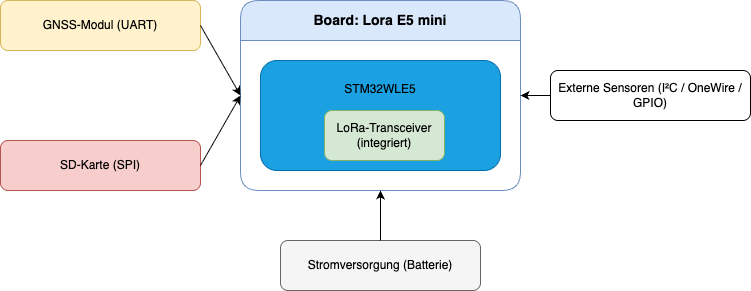
\includegraphics[scale=.5]{figures/diagrams/Architekturdiagramm_LoraE5mini.png}
\caption{Systemarchitektur Lora E5 mini}
\label{fig:systemarchtektur-lora-e5-mini}
\end{figure}

Das Heltec LoRa V2 hingegen basiert auf einem ESP32-Mikrocontroller, wie in Abbildung \ref{fig:systemarchtektur-heltec-lora-v2} zusehen, ist bei diesem Board der LoRa-Chip separat angebunden. Der ESP32 bietet zudem umfangreiche Energiesparmodi, insbesondere den Deep-Sleep-Modus, wodurch sich verschiedene Ansätze zur Laufzeitoptimierung evaluieren lassen. Zusätzlich verfügt das Board über integrierte Peripheriekomponenten wie ein OLED-Display, das für Debugging und Testzwecke nützlich war. 

\begin{figure}[H]
\centering
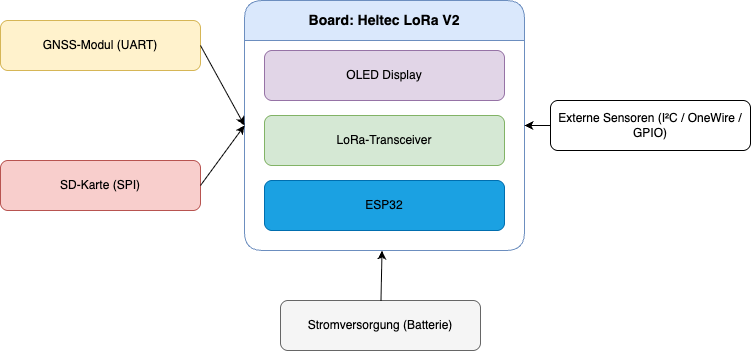
\includegraphics[scale=.5]{figures/diagrams/Architekturdiagramm_ESP32.png}
\caption{Systemarchitektur Heltec LoRa V2}
\label{fig:systemarchtektur-heltec-lora-v2}
\end{figure}

Neben den Entwicklungsboards bildeten zwei weitere Komponenten zentrale Elemente der Hardwarearchitektur:  
\begin{itemize}
    \item \textbf{GPS-Modul:} Das GNSS-Modul dient primär der Positionsbestimmung und stellt die wesentlichen Geodaten für das Tracking bereit. Darüber hinaus wird die vom Modul gelieferte Zeitinformation als Zeitbasis für das Gesamtsystem genutzt, wodurch das Gerät ohne separate Echtzeituhr über eine zuverlässige Zeitreferenz verfügt. 
    \item \textbf{SD-Karte:} Die SD-Karte wird einerseits für das lokale Logging der Messdaten eingesetzt, sodass auch bei temporären Übertragungsproblemen eine vollständige Aufzeichnung gewährleistet bleibt. Andererseits speichert sie persistente Systemparameter, wie das aktuell konfigurierte Sendeintervall sowie den LoRaWAN-Nonce-Wert, der für die sichere Teilnahme am Netzwerk erforderlich ist. Dadurch lassen sich sowohl Sicherheit als auch Reproduzierbarkeit der Übertragungen erhöhen.
\end{itemize}

Die Grundarchitektur der Prototypen sah damit eine zentrale Mikrocontroller-Einheit mit angebundener Peripherie vor. Das GPS-Modul wurde über eine UART-Schnittstelle angeschlossen, während die SD-Karte über SPI verbunden war. Weitere Sensoren, wie beispielsweise Temperatursensoren, konnten über gängige Schnittstellen wie I\textsuperscript{2}C oder OneWire ergänzt werden. 

Die Entwicklung erfolgte auf Basis von Entwicklungsboards in Verbindung mit Breadboards, wodurch eine schnelle Iteration und flexible Erweiterbarkeit möglich war. Auf die Anfertigung eigener Leiterplatten wurde im Rahmen des Proof-of-Concepts bewusst verzichtet, da der Fokus auf Funktionalität und Modularität lag und nicht auf der finalen Produktoptimierung.